\chapter{Fundamentação Teórica} \label{cha:fundamentacao}

A seguir são apresentados conceitos, visões e abordagens de autores quanto aos temas necessários para o entendimento desse trabalho, bem como a descrição das tecnologias utilizadas para o desenvolvimento da solução Topin.

\section{Sistema de Informação}

Para \citeonline{stair} um Sistema de Informação é composto por um conjunto de componentes (Figura \ref{fig:sistema-de-informacao}) inter-relacionados com o intuito de coletar, manipular, armazenar e disseminar dados e informações, além de fornecer um mecanismo de realimentação para atingir um objetivo.

\begin{figure}[H]
\caption{Componentes De Um Sistema De Informação}
\centering
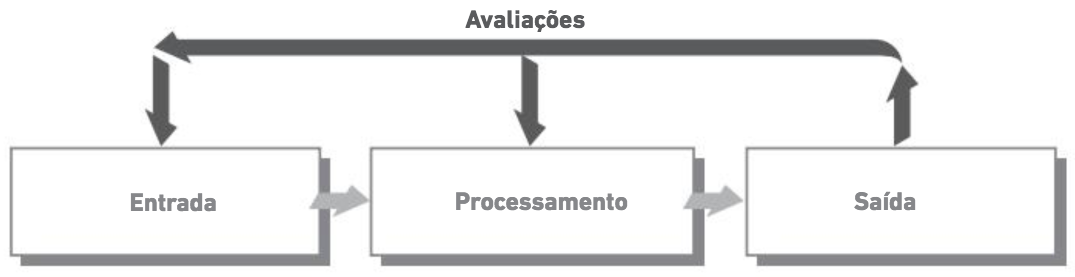
\includegraphics[width=1\textwidth]{imagens/sistema-de-informacao.png}
\legend{Fonte: Cengage Learning}
\label{fig:sistema-de-informacao}
\end{figure}

\subsection{Sistema Inteligente de Transporte}

Segundo \citeonline{figueiredo} os Sistemas Inteligentes de Transporte são uma tendência mundial em constante crescimento que entrou em evidência após sociedade moderna dar mais importância a mobilidade e, com isso, os ITS passaram a contemplar os setores públicos e privados colocando em destaque assuntos de índole política, econômica e social.

Ainda sobre a visão de \citeonline{figueiredo} os ITS pretendem conciliar a cultura, a indústria, a econômica, a natureza, o ambiente e por fim o estilo e qualidade de vida do ser humano. A definição dos ITS não apenas revoluciona a interação entre pessoas e veículos, como também possibilita o desenvolvimento de novas relações espaciais e, por este motivo, viabiliza a comunicação entre veículos e pessoas, constituindo uma sociedade avançada baseada em informação. 

De acordo com a \citeonline{iso_10992} os ITS se dividem nas seguintes categorias:

\begin{lista}
\item Gerenciamento de tráfego;
\item Informações aos usuários;
\item Gerenciamento das rodovias;
\item Sistemas de condução assistida de última geração;
\item Gerenciamento de veículos comerciais;
\item Gerenciamento do transporte público;
\item Pagamento eletrônico;
\item Respostas a incidentes e desastres.
\end{lista}

Das oito categorias abordadas pelos ITS, os sistemas de informações aos usuários vem sendo desenvolvido em várias cidades brasileiras \cite{revista_opara}. Nesta categoria encontram-se aplicações que disponibilizam informações antes do deslocamento, informações durante o deslocamento e serviços pessoais de informação para os usuários.

\subsection{Sistema de Informação Geográfica}

Os Sistemas de Informação Geográfica (em inglês \textit{Geographic Information System} - GIS) se tornaram um importante instrumento para a resolução de problemas relacionados ao transporte. Inúmeros estudos se utilizam de GIS no planejamento, gestão, operação e análise de sistemas de transporte, as aplicações dos Sistemas de Informação Geográfica nos transportes são diversificadas, entre elas pode-se citar o transporte coletivo urbano, rodoviário, de carga e engenharia de tráfego. \cite{dantas}

Para \citeonline{rose} os Sistemas de Informação Geográfica são a melhor ferramenta para solucionar problemas de organização de dados em modelos espaciais. Inúmeras empresas privadas e órgãos governamentais tomam decisões relacionadas ao planejamento com base em um GIS, utilizando de seus recursos em relação a ferramentas de gerenciamento, bancos de dados e processamento de dados. os Sistemas de Informação Geográfica também tem sido elemento chave para aprimorar o gerenciamento de transportes existentes.

\subsection{Sistema de Posicionamento Global}

Para \citeonline{vazquez} os Sistemas de Posicionamento Global (em inglês \textit{Global Positioning System} - GPS) funcionam de modo a permitir que se determine posições precisas para cada ponto ao redor do globo terrestre, facilitando assim a possibilidade de inserirmos dados associados a um ponto no espaço, como por exemplo, determinar a localização exata de um hotel ou, inclusive, a localização em tempo real de um objeto em movimento.

\section{Engenharia de Sofware}

Para \citeonline{sommerville} a Engenharia de Software é uma disciplina da engenharia que aborda todos os aspectos da produção de um \textit{software} desde os estágios iniciais da especificação do sistema até a sua manutenção, apesar de não se restringir as atividades de implementação, dado que também se preocupa com o gerenciamento de projetos e a criação de novas ferramentas, métodos e teorias quando não houver alternativa viável, para suportar a produção do \textit{software}, entretanto existem 4 atividades fundamentais para a Engenharia de Software:

\begin{lista}
\item Especificação do \textit{software};
\item Desenvolvimento de \textit{software};
\item Validação de \textit{software};
\item Evolução do \textit{software}.
\end{lista}

Segundo \citeonline{rezende} a Engenharia de Software é um conjunto de métodos para implementação e manutenção de aplicações segmentadas, que estejam de acordo com as características abaixo:

\begin{lista}
\item Processo dinâmico, integrado e inteligente de soluções tecnológicas;
\item Adequação aos requisitos funcionais do negócio do cliente e seus respectivos procedimentos pertinentes;
\item Efetivação de padrões de qualidade, produtividade e efetividade em suas atividades e produtos;
\item Fundamentação na Tecnologia da Informação disponível, viável, oportuna e personalizada;
\item Planejamento e gestão de atividades, recursos, custos e datas.
\end{lista}

\subsection{Análise de Requisitos}

Para a Engenharia de Software a documentação e levantamento dos requisitos é um dos problemas básicos encontrados durante o planejamento do desenvolvimento de um produto de \textit{software}, porque se o levantamento é feito da forma correta, os requisitos implícitos, que são os requisitos cobrados por clientes que não foram informados no levantamento de requisitos, são minimizado de modo a evitar problemas no andamento da implementação do sistema, pois requisitos não documentos dificilmente entraram no desenho do produto ocasionando em alterações não desejadas e inesperadas, bem como a insatisfação do cliente. \cite{padua}

Os requisitos de \textit{software} são as funções ou características pertencentes a um \textit{software}, requisitadas pelo cliente ou usuário para resolver um problema ou atingir um objetivo. \cite{eee1990}

O valor de um produto de \textit{software} é proveniente de suas características ou requisitos. Ao se trabalhar com desenvolvimento de sistemas esses requisitos são divididos em duas categorias: requisitos funcionais e requisitos não funcionais. \cite{padua}

\subsubsection{Requisitos Funcionais}

Os requisitos funcionais podem ser definidos como as funções ou atividades que são ou viram a ser desempenhadas por um sistema computacional. Estes devem ser definidos de forma clara e posteriormente relatados explicitamente. \cite{sommerville}

\subsubsection{Requisitos Não Funcionais}

Para \citeonline{cysneiros} os requisitos não funcionais, diferentemente dos requisitos funcionais, não estão relacionados a uma função que o sistema deve desempenhar, mas sim aos comportamentos e restrições que este \textit{software} deve satisfazer.

\subsection{Linguagem de Modelagem Unificada}

Linguagem de Modelagem Unificada (em inglês \textit{Unified Modeling Language} - UML) é uma linguagem gráfica para elaboração de artefatos que irão permitir a visualização, especificação, construção e documentação de artefatos de sistemas complexos de \textit{software}. A UML é um forma de garantir a padronização no momento de preparação de planos de arquitetura de projetos de sistemas, incluindo aspectos conceituais tais como processos de negócios e funções do sistema, além de itens concretos como as classes escritas em determinada linguagem de programação, esquemas de bancos de dados e componentes de \textit{software} reutilizáveis.\cite{uml}

Como pode ser visto na Figura \ref{fig:uml}, a UML é formada por um conjunto de diagramas que podem ser classificados em três categorias:

\begin{lista}
\item \textbf{Diagramas de Estruturas:} Descreve o sistema de forma estática, abordando as partes referentes a objetos, classes, atributos, operações, bem como os relacionamentos entre si.
\item \textbf{Diagramas de Comportamento:} Descreve o funcionamento dos módulos e os processos do negócio que possuem relação com o sistema.
\item \textbf{Diagramas de Interação:} Subgrupo dos diagramas de comportamento responsável pela descrição das interações entre os objetos.
\end{lista}

\subsubsection{Diagrama de Casos de Uso}

De acordo com \citeonline{guedes} o diagrama de casos de uso tem por definição o objetivo de permitir que qualquer pessoa com o mínimo de conhecimento sobre o problema possa compreender o comportamento externo do sistema pela perspectiva dos usuários, ou seja, apresenta uma visão geral das funcionalidades que o sistema deve oferecer aos usuários, sem considerar os detalhes de implementação.

\begin{figure}[H]
\caption{Visão Geral da UML}
\centering
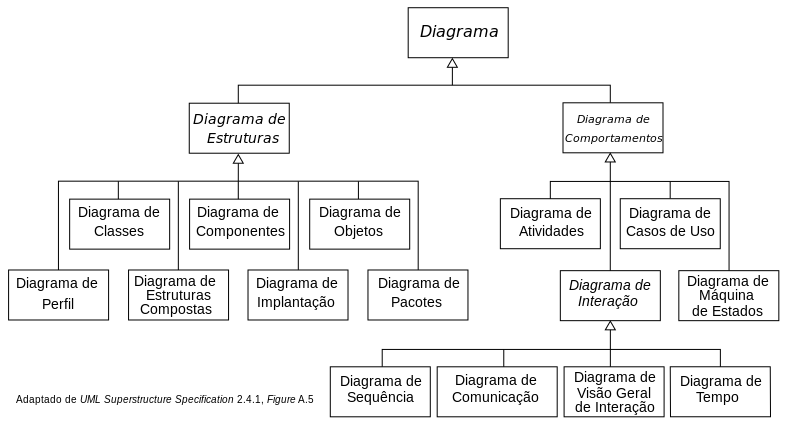
\includegraphics[width=1\textwidth]{imagens/uml.png}
\legend{Fonte: Wikimedia Commons}
\label{fig:uml}
\end{figure}

\subsubsection{Modelo Entidade-Relacionamento}

O modelo entidade-relacionamento (MER) é representado visualmente por meio de um diagrama entidade-relacionamento (DER). O MER é considerado um padrão para a modelagem conceitual de bancos de dados desde sua criação em 1976, por Peter Chen.\cite{heuser}

O MER tem o objetivo de representar de forma abstrata um banco de dados, interessam-se apenas os objetos sobre os quais existe a necessidade de armazenar as informações. Com ele é possível representar as entidades, relacionamentos e cardinalidades de todos os objetos que compõem o \textit{software} objeto deste trabalho e, a partir dele, é possível implementar o banco de dados que será utilizado neste projeto.\cite{heuser}

\subsection{Arquitetura de Software}

De acordo com \citeonline{bass} a arquitetura de \textit{software} de um sistema computacional é formado por uma ou mais estruturas que compreendem todos os elementos do \textit{software}, bem como suas propriedades visíveis externamente e o modo como estão interligadas.

Para \citeonline{bass} a importância da arquitetura de \textit{software} para o sistema se da por meio de 3 tópicos principais, são estes:

\begin{lista}
\item \textbf{Comunicação entre as partes interessadas}. A arquitetura de \textit{software} representa uma abstração comum de um sistema que a maioria das partes interessadas no sistema podem usar como base para entendimento, negociação, consenso e comunicação.
\item \textbf{Decisões antecipadas de design}. A arquitetura de \textit{software} manifesta as primeiras decisões de projeto sobre um sistema, e essas ligações iniciais carregam um peso muito grande em relação ao desenvolvimento restante do sistema, sua implantação e sua vida de manutenção. Como também é a primeira oportunidade pra avaliar o que será desenvolvido e analisar o melhor caminho a ser desempenhado pela equipe.
\item \textbf{Modelo genérico}. A arquitetura de \textit{software} constitui um modelo relativamente pequeno, genérico e de fácil compreensão que representa como um sistema é estruturado e como seus elementos trabalham em conjunto, bem como pode ser reproduzido e aplicado a outros sistemas.
\end{lista}

Para \citeonline{pressman} arquitetura não é o \textit{software} operacional. Pelo contrário, é uma representação que permite a um engenheiro de \textit{software}:

\begin{lista}
\item Analisar a eficiência do projeto em atender aos requisitos levantados.
\item Considerar as alternativas de arquitetura em um estágio em que fazer mudanças no projeto ainda é processo relativamente fácil e menos custoso.
\item Reduzir os riscos associados ao desenvolvimento do \textit{software}.
\end{lista}

\subsection{Interface de Programação de Aplicativos}

\citeonline{masse} afirma de forma sucinta que uma Interface de Programação de Aplicativos (em inglês \textit{Application Programming Interface - API}) é um modo de expor um conjunto de dados e funções para facilitar as interações entre programas de computador e permitir que troquem informações.

\subsubsection{Transferência de Estado Representacional}

\citeonline{fielding} definiram os princípios da arquitetura moderna da internet desenvolvendo um modelo de transferência de dados na \textit{web}, nomeado de Transferência de Estado Representacional (em inglês \textit{Representational State Transfer - REST}), este modelo consiste em um conjunto coordenado de restrições arquiteturais que tenta minimizar a latência e a comunicação de rede, maximizando ao mesmo tempo a independência e a escalabilidade da implementação dos componentes.

\subsubsection{Protocolo de Transferência de Hipertexto}

Para \citeonline{fielding-http} O Protocolo de Transferência de Hipertexto (em inglês \textit{Hypertext Transfer Protocol - HTTP}) é um protocolo em nível de aplicativo para sistemas de informações hipermídia distribuídos e colaborativos. É um protocolo genérico, sem estado, que pode ser usado para muitas tarefas além de seu uso para hipertexto, como servidores de nomes e sistemas de gerenciamento de objetos distribuídos, através da extensão de seus métodos de solicitação, códigos de erro e cabeçalhos.

{\renewcommand{\arraystretch}{2}
\begin{table}[H]
\centering
\caption{Principais Métodos do Protocolo HTTP}
\label{tab:metodos-http}
\begin{tabular}{ l | p{13.5cm} }
\hline
\textbf{Método} & \textbf{Função} \\
\hline
GET & Recuperar os dados de um recurso. \\ \hline
POST & Adicionar um novo recurso. \\ \hline
PUT & Atualizar os dados de um recurso. \\ \hline
PATCH & Atualizar apenas alguns dados de um recurso. \\ \hline
DELETE & Apagar um recurso. \\ \hline
\end{tabular}
\legend{Fonte: Autor}
\end{table}

\subsection{Métodos Ágeis}

Os métodos ágeis são métodos de desenvolvimento incremental baseados na entrega de pequenos incrementos, onde novas versões do sistema são implementadas e fornecidas aos clientes em prazos curtos, geralmente, de duas a três semanas. Eles colocam a participação do cliente como essencial no processo de desenvolvimento do \textit{software} no intuito de obter um \textit{feedback} rápido sobre as mudanças e requisitos do sistema. Assim, podem minimizar a documentação utilizando-se de uma comunicação informal, ao invés de reuniões formais com documentos escritos. \cite{sommerville}

A filosofia dos métodos ágeis é refletida através  do manifesto ágil que foi criado por grande parte dos principais desenvolvedores desses métodos, esse manifesto afirma que um método ágil deve valorizar os seguintes aspectos:

\begin{lista}
\item Valorizar os indivíduos e as suas interações acima dos processos e ferramentas;
\item Valorizar mais o \textit{software} em funcionamento do que uma documentação abrangente;
\item Valorizar a colaboração do cliente em relação à negociação de contratos;
\item Valorizar a capacidade de responder a mudanças ao invés de seguir um plano.
\end{lista}

\subsubsection{Scrum}

O Scrum aborda todas as suas práticas em uma estrutura de processo incremental e iterativo, como pode ser visto na Figura \ref{fig:scrum} o ciclo maior representa a \textit{Sprint Retrospective} em que demonstra uma iteração das atividades de desenvolvimento que ocorrem uma após a outra em pequenos intervalos de tempo, geralmente entre duas e quatro semanas. A saída de cada iteração consiste em um incremento do produto. O círculo menor representa as reuniões diárias (em inglês \textit{Daily Scrum}) que ocorrem todos os dias durante a iteração, onde todos os membros da equipe se reúnem para discutir as atividades em desenvolvimento e efetuar as modificações apropriadas, se necessário. O ciclo de iterações deve ser repetido até que o objetivo do projeto tenha sido alcançado ou não esteja mais sendo financiado. \cite{schwaber}

\begin{figure}[H]
\caption{Ciclo de Vida do Scrum}
\centering
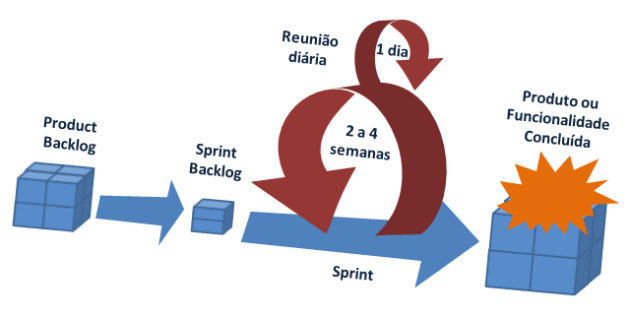
\includegraphics[width=0.9\textwidth]{imagens/scrum.png}
\legend{Fonte: Mind Master}
\label{fig:scrum}
\end{figure}

\subsubsection{Kanban}

Segundo os autores \citeonline{kniberg} o Kanban é aplicado de um modo em que as atividades que estão em processo de desenvolvimento devem ser limitadas e novas atividades só podem ser desempenhadas quando uma das atividades que estão em andamento são entregues ou movidas para uma etapa diferente do processo. O Kanban determina que um sinal visual deve ser produzido na tentativa de indicar que um novo trabalho pode ou não ser colocado em desenvolvimento e, assim, determinar se o trabalho atual estará em conformidade com o limite de acordado.

\begin{figure}[H]
\caption{Exemplo de Kanban}
\centering
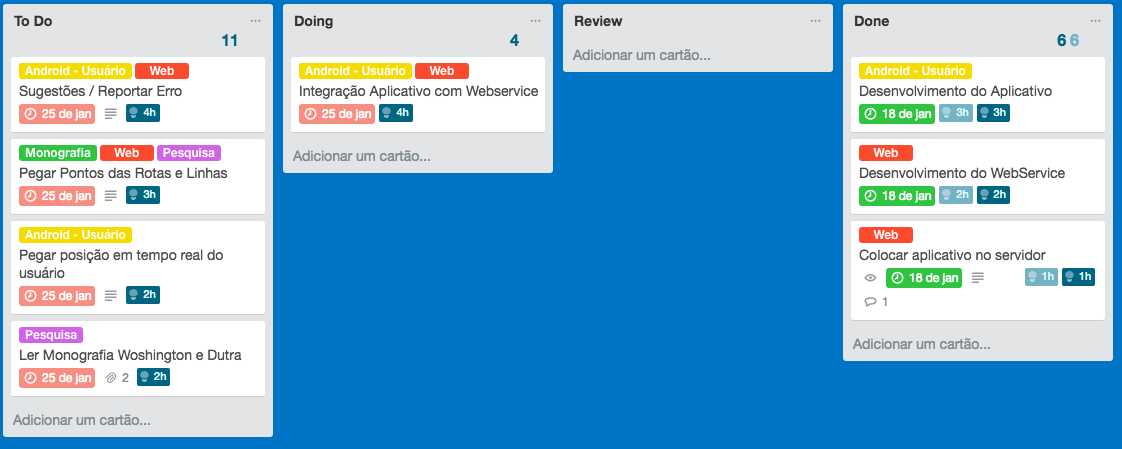
\includegraphics[width=0.9\textwidth]{imagens/kanban.png}
\legend{Fonte: Autor}
\label{fig:kanban}
\end{figure}